%Approach
\chapter{Approach}
As briefly discussed earlier, our approach is to train a seasonal ARIMA model for a base level of forecasting.  The residual forecasting errors of this approach are then run through an activity recognition algorithm to produce a set of models corresponding to instances where the ARIMA model mis-forecasts.  Final forecasting is then determined by combining the forecasts of all activity models and the background seasonal ARIMA model using a Bayesian combined predictor.  The entire approach is unsupervised.

While research has shown that univariate ARIMA models outperform multivariate ARIMA models for forecasting, we believe it possible that activity models will perform better when the data of spatially local sensors (neighbors) are included.  For each sensor, knowledge of its neighbors allows for reduced computation time when computing what sensors are optimal for each activity.  Thus, for our approach to be unsupervised, it is necessary to calculate sensor neighbors.

This section outlines all aspects of our approach.  First we describe a method to calculate the temporal and spatial correlations of the data observed by the sensors giving sensor neighbors.  Following this is a discussion on fitting a seasonal ARIMA model.  Then we describe a couple of potential approaches to model activities.  Finally we discuss prediction and performance calculations.

%Spatial and Temporal Correlation of sensors
\section{Spatial and Temporal Correlation of Sensors}
Determining how sensors are correlated allows for unsupervised approaches to searching for the optimal set of sensors which make up an activity.  This correlation is determined by calculating Pearson's correlation for each pair of sensors at a given time offset.  For reference Pearson's correlation is:
\begin{equation}
\label{eq:pearson}
C_{pearson}(a, b) = \frac{E(ab) - E(a)E(b)}{\sqrt{E(a^{2})-E^{2}(a)}\sqrt{E(b^{2})-E^{2}(b)}}
\end{equation}

\noindent
where $E(a)$ is the expected value of the random variable $a$.

Converting this formula to binary data and applying a time offset $\delta$ gives
\begin{equation}
\label{eq:correlation}
C_{binary}(a, b;\delta) = \frac{E(x_{a}x_{b}) - E(x_{a})E(x_{b})}{\sqrt{E(x_{a})-E^{2}(x_{a})}\sqrt{E(x_{b})-E^{2}(x_{b})}}
\end{equation}

\begin{figure}[t]
\begin{center}
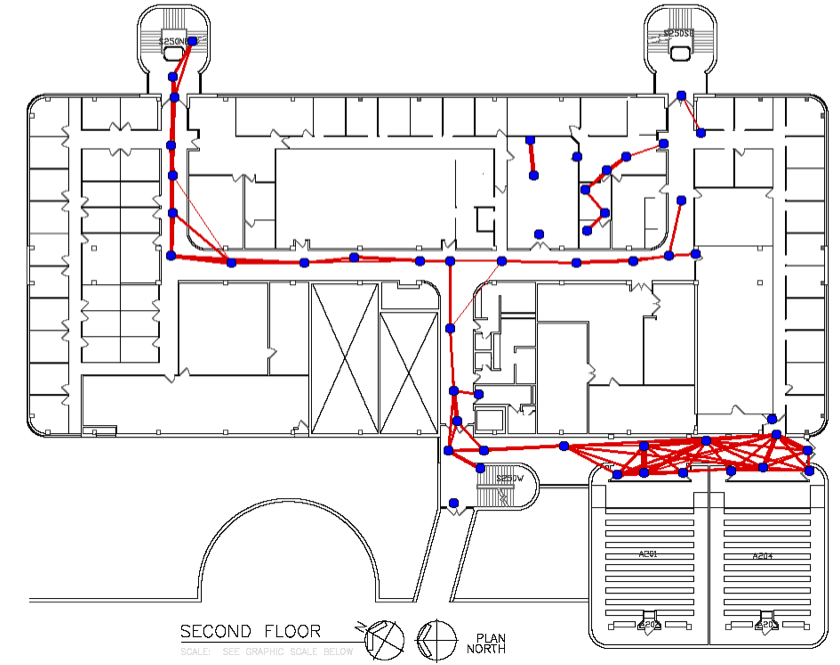
\includegraphics[width=0.8\textwidth]{brown_correlation.png}
\end{center}
\caption{Pairwise sensor correlation}
\label{fig:brown_correlation}
\end{figure}

\noindent
where the values for $x_{b}$ are always at a time offset of $\delta$ in the future of $x_{a}$.  Thus if given $x_{a}^{(i)}$ then calculations are performed with $x_{b}^{(i + \delta)}$.

Next the maximum value of $C_{binary}$ for all $\delta$ is found
\begin{equation}
\label{eq:max_correlation}
\arg\max_{\delta} \  C_{binary}(a, b;\delta) \quad \forall \delta \in \{1, 2, ..., M\}).
\end{equation}

In practice, as a way to reduce computation time, the calculation can be performed with a much smaller maximum $\delta$ than $M$.  The returned maximum value of $\delta$ for each pair of sensors is a good indicator of travel time between the two sensors.  This information is useful for determining what sensors to use when calculating activities.

Figure ~\ref{fig:brown_correlation} shows an example of this approach.  This figure displays the maximum pairwise sensor correlations across a $\delta$ of up to 10 seconds.   The values were then thresholded to prevent displaying every line between two sensors.  The line thickness represents the correlation value.  While the pairings are not perfect in all places, this figure does show the potential of this approach.  

%Background Model
\section{Seasonal ARIMA Model}
The seasonal ARIMA model has two important roles in this work.  One role is its direct predictive capabilities.  The other role is for the determination of activities.  The residual data created from subtracting the current observations from seasonal ARIMA forecasts is used as the basis for activities.  This section briefly outlines the steps necessary to fit a seasonal ARIMA model for our problem.  

\begin{figure}[t]
\begin{center}
\subfloat[][Vehicle counts] {
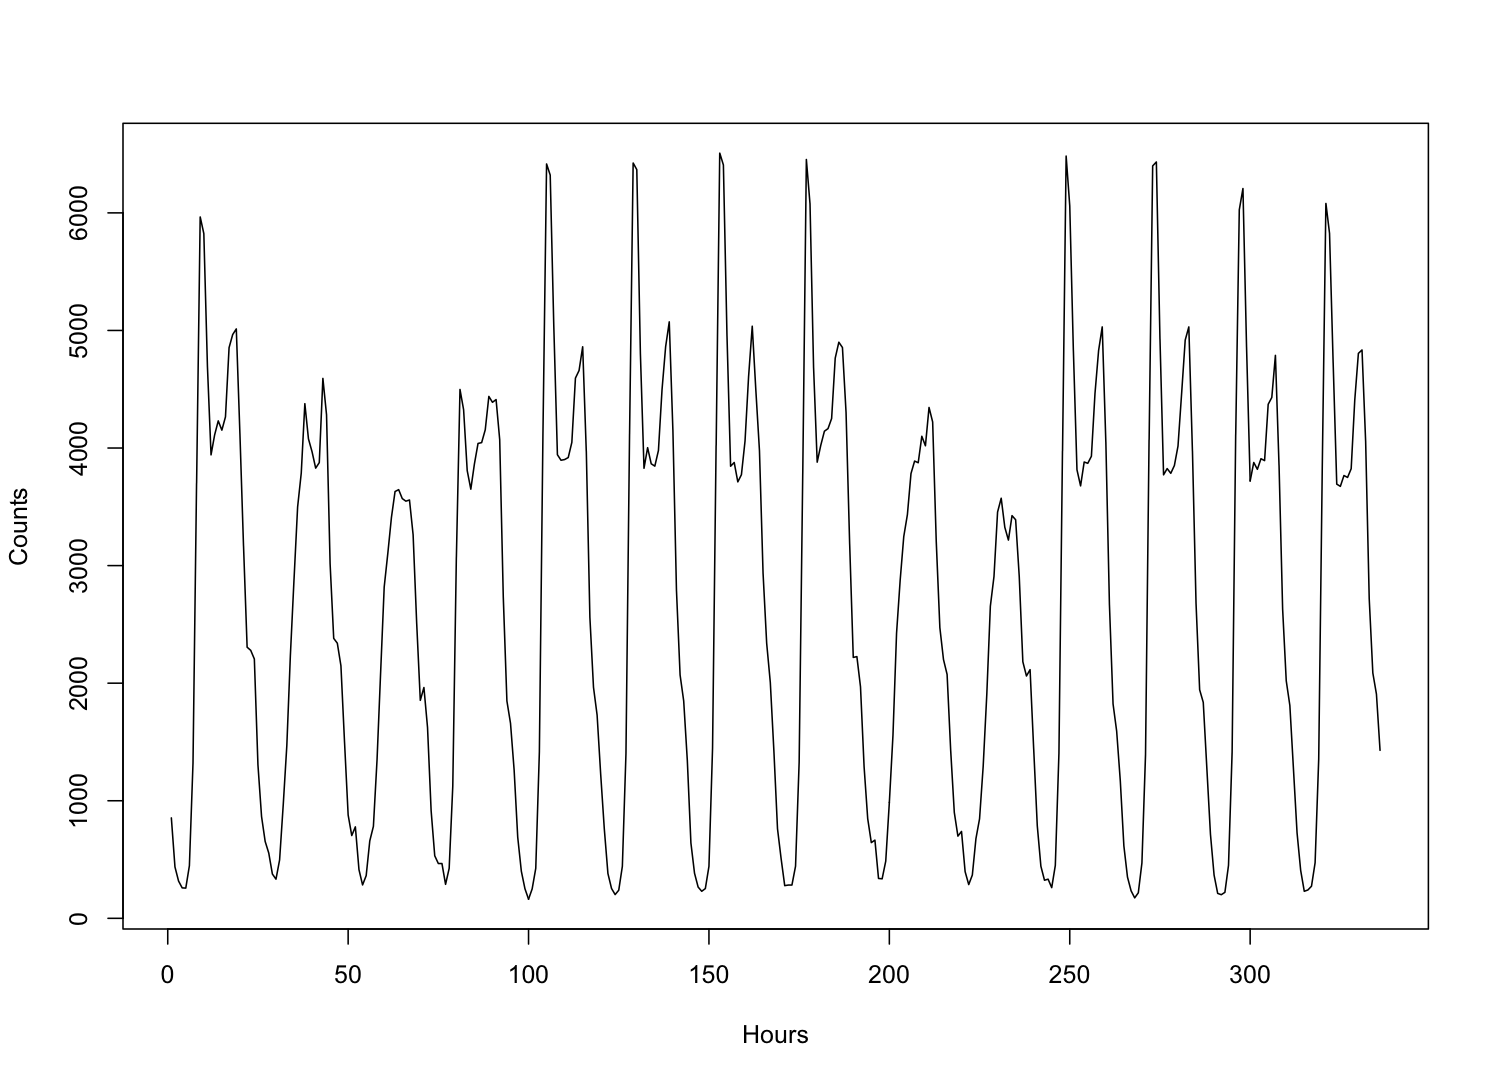
\includegraphics[width=0.45\textwidth]{counts.png}
\label{fig:counts}
}
\subfloat[][Autocorrelation of vehicle counts] {
\includegraphics[width=0.45\textwidth]{acf_counts.png}
\label{fig:acf_counts}
}
\end{center}
\caption{Counts and autocorrelation over a two week period.}
\label{fig:raw_data}
\end{figure}


\subsection{Fitting a Seasonal ARIMA}
The underlying math of ARMA models stems from a linear filter operating on input from a stationary stochastic process.  ARIMA models were created to handle non-stationary data by differencing the data to induce stationarity.  Thus, a necessary step in fitting a ARIMA model to the data is first to determine the steps necessary to make the time series weakly stationary.  For a time series to be weakly stationary two conditions must be satisfied: The expected value of $x^{(t)}$ is the same for all $t$ and the covariance between any two observations depends only on the lag.  

In general it is difficult to prove stationarity, but there exists a number of methods which assist in determining if a time series is close enough to stationary to be modeled by an ARMA model.  Visual inspection of both the raw data and the autocorrelation function is a useful tool to test for stationarity.  Figure~\ref{fig:raw_data} shows the raw counts and autocorrelation values at hourly lags of vehicle counts for one sensor over a two week period.  The data shows no constant mean and thus can not be stationary.  The graph of autocorrelation values shows local peaks every 24 hours with a significant peak at one week of lag (168 hours).

Intuitively a one week seasonal difference should yield a stationary time series and visually, outside of an anomalous reading, Figure~\ref{fig:acf_lag} shows such stationarity.  Applying the Kwiatkowski-Phillips-Schmidt-Shin (KPSS) \cite{Kwiatkowski1992} test for stationarity on the seasonally differenced data confirms the visual inspection.  Using R's implementation of KPSS gives a p-value greater than 0.1.  This is significantly higher than the standard value to reject the stationarity hypothesis of 0.05.  

\begin{figure}[t]
\begin{center}
\subfloat[][Seasonal difference counts] {
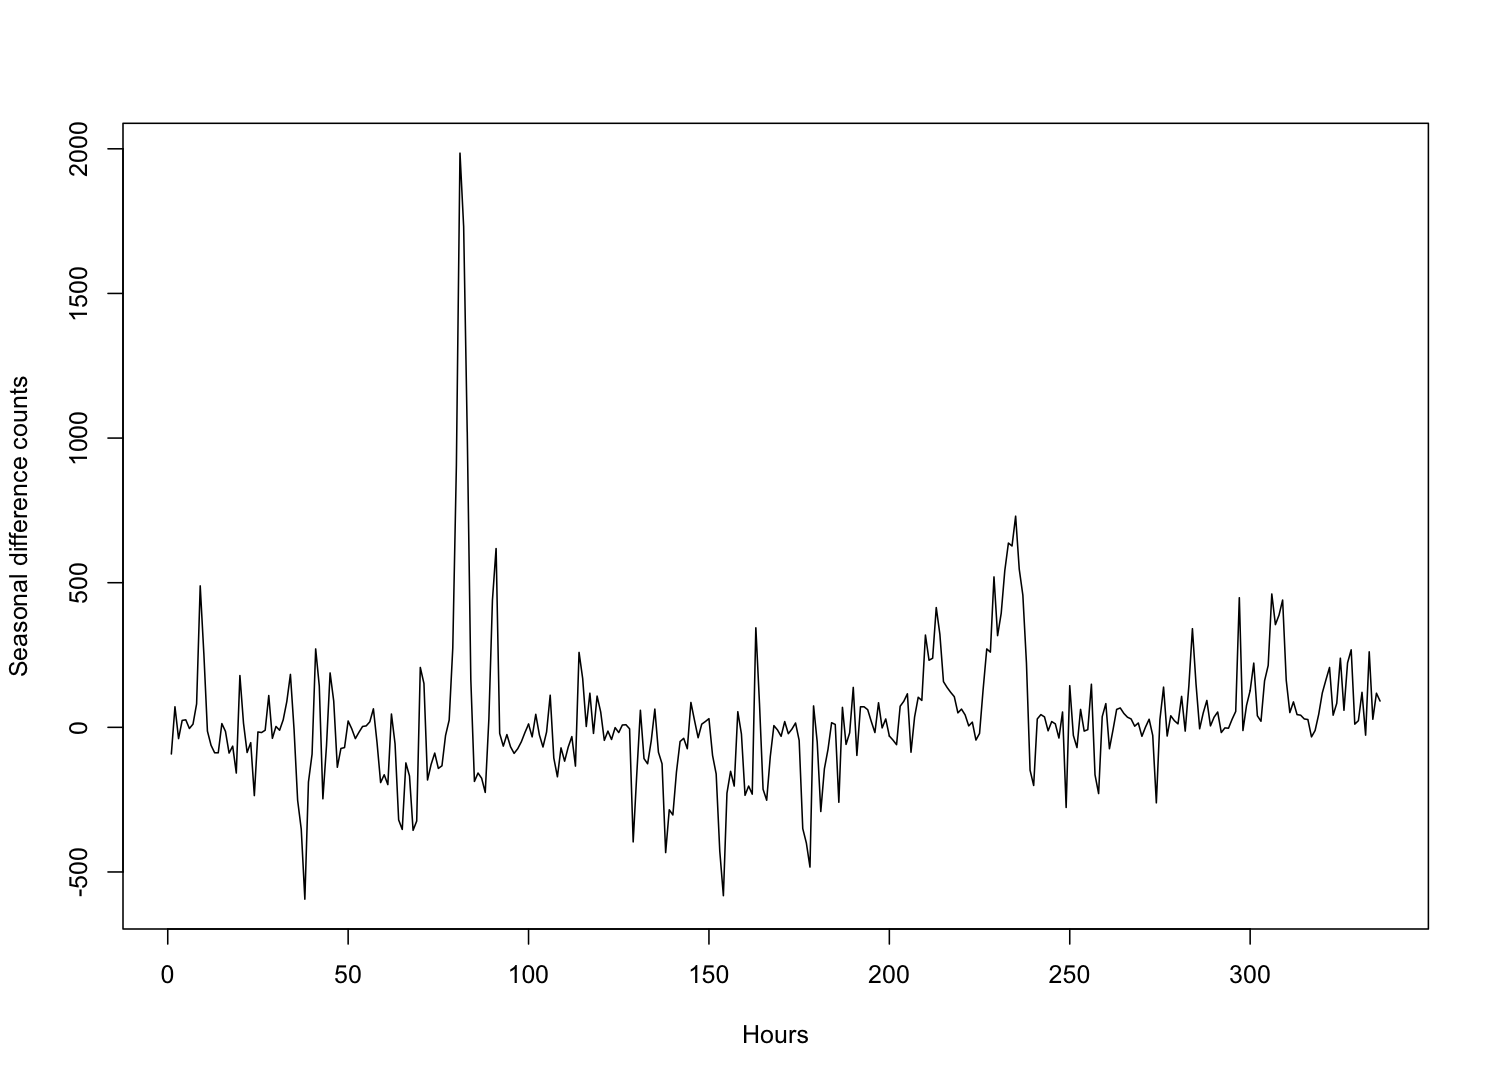
\includegraphics[width=0.45\textwidth]{lag_counts.png}
\label{fig:acf_counts}
}
\subfloat[][Autocorrelation of seasonal difference counts] {
\includegraphics[width=0.45\textwidth]{acf_lag.png}
\label{fig:acf_lag}
}
\end{center}
\caption{One week seasonal difference counts and autocorrelation over a two week period.}
\label{fig:lag_data}
\end{figure}

Most of the input parameter values for seasonal ARIMA models tend to be 0, 1, 2, or 3 \cite{Box2008}.  Due to this small range of input values the total input space is relatively small (Six parameters with four possible values equates to $4^6 = 4096$) allowing us to apply a brute-force search for the best model.  Model performance is determined by the Akaike information criterion (AIC) \cite{akaike1974}.  Our optimal model is a seasonal ARIMA $(1,0,1)(0,1,1)_{168}$.  

\begin{figure}[h]
\begin{center}
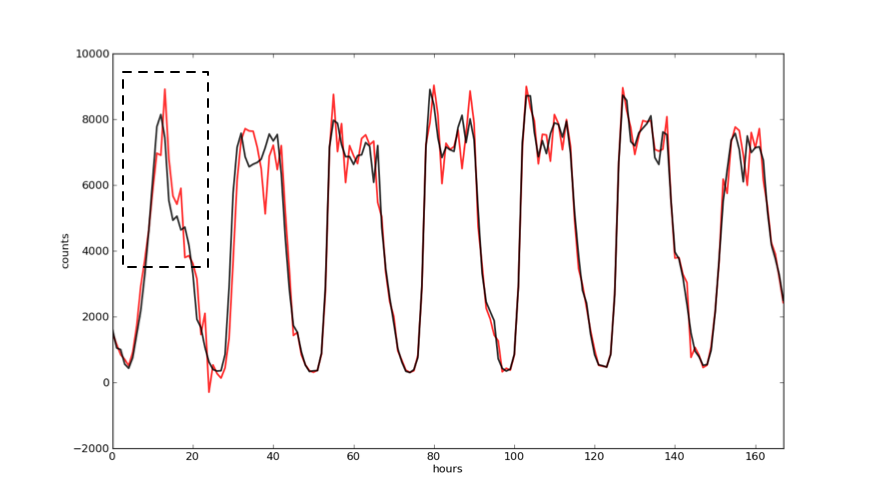
\includegraphics[width=0.8\textwidth]{broncos_predicted.png}
\end{center}
\caption{One-step ahead prediction for a sample week.  Black line is original data.  Red line is forecasted data.  Dotted box shows an example of mis-forecasting due to a broncos game.}
\label{fig:arima_prediction}
\end{figure}

Figure~\ref{fig:arima_prediction} shows an example of one-step ahead prediction performed on a sample week of test data.  The dotted line boxes a time when a Broncos game was occurring.  Forecasting during the Broncos game was initially low while traffic was unusually high as people were traveling to the game and then too high for much of the duration of the game.  This pattern of mis-forecasting is inline with the pattern demonstrated in Figure~\ref{fig:broncos_residual}.  The mean absolute percentage error (MAPE) for this week was approximately 8.2\%.  This MAPE is close to the results from other authors on other vehicle traffic datasets \cite{Williams2003,Smith1997}.  

%Activity Recognition
\section{Activity Recognition}
This section first details some of the challenges to obtaining training data for activities in an unsupervised manner.  Next we describe two algorithms used to cluster activities from the training dataset.  Finally we introduce a new measure of the length of time required to classify activities.

\subsection{Training Data}
Segmenting a time series of data which will be used to train activities is an important problem.  A time series that is too long may encompass multiple activities, while one that is too short will not adequately describe an entire activity.  Factors that need to be considered are what length of time each time series will cover, the features included in the time series and if the time series will overlap.  

The problem of unsupervised time series data segmentation for activity recognition is not commonly discussed in the literature.  In much of the activity recognition literature the problem is not applicable as data either splits naturally (such as RFID item usage data) or is supervised (such as human wearable accelerometers).

One approach we have implemented involves sliding a fixed window over the residual data to parse out local time series of maximum deviation.  The problem with this approach is that it does not consider windows of different lengths.  As an initial solution to this problem, we will repeat this process with multiple window lengths and include all time series as valid training data.  This approach is not ideal and we will continue to search for a better solution to isolate residual data associated with activities.

%\subsection{Dimensionality Reduction}
%It is possible that activities will require a large number of sensors to model.  Reducing the dimensionality of the observation space can be beneficial for both computational and accuracy reasons.  Below are a few of the ways in which we have attempted to reduce the dimensionality of the activity time series inputs.

%\subsubsection{Clustering}
%In this approach data is broken up into windows of m seconds long $d = \{x^{(i)}, x^{(i + 1)}, ..., x^{(i + m)}\}$.  Each data point is a vector from the nearest n sensors as chosen by the temporal correlation scores of the data.  Each dimension in $d$ is then summed to produce a total data vector for each time window.  

%Each time window from $d$ is used as the input into a clustering algorithm.  Due to this work being completly unsupervised, it is necessary to find a clustering score that does not rely on labeled data.  The silhouette score \cite{Kaufman1990} is a scoring metric that fits this criteria.  It simultaneously attempts to minimize intra-cluster distance while maximize inter-cluster distance.  The silhouette score is:

%\begin{equation}
%\label{eq:silhouette}
%S_{sil}(i) = \frac{\min(B(i, :)) - A(i)}{\max(A(i), \min(B(i, :)))}
%\end{equation}

%Where $A(i)$ is the average distance from the $ith$ point to the other points in its cluster, and b(i, k) is the average distance from the ith point to points in another cluster k.

%Clustering is then performed using either agglomerative or k-means clustering algorithms.  For each observation vector features would be the classified cluster for every observation vector.

%\subsubsection{Probabilistic Latent Semantic Analysis}
%Another approach that has we have explored with good preliminary results is probabilistic latent semantic analysis  (PLSA) \cite{Hofmann1999,Hofmann1999a}.  PLSA is a statistically founded approach to information retrieval and automatic indexing for document analysis.  It attempts to determine a best set of possible latent classes which can describe all documents from a corpus.  In the domain of document analysis these latent classes are typically interpreted as topics.

%Mapping PLSA from the document domain to the domain of this work is done by assuming that all data $x$ is the basis of a corpus.  Data is then separated based on fixed time windows.  Each section of separated data is equivalent to a "document."  From there, a count of the words which make up that document are extracted.  In our case, these words are either sensor reading or an extracted feature.  

%The results of PLSA are a set of latent classes which are able to describe the corpus of documents.  An example in the document analysis domain might be using all articles from the magazine "Science" as a corpus.  The extracted latent classes may be described as "astronomy", "biology", "physics," etc.  With these classes calculated, any new document is described as a combination of these latent classes.  A new article on how relativity works inside a black hole will be described by astronomy and physics classes with little to no biology.  

%\begin{figure}[t]
%\begin{center}
%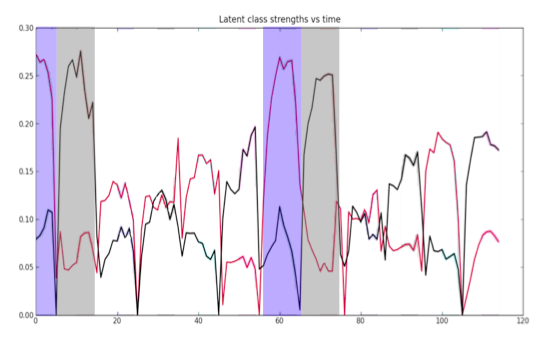
\includegraphics[width=0.8\textwidth]{plsa.png}
%\end{center}
%\caption{Graph of projection strengths over time in a simulated noisy environment with two meetings.  The read and black lines correspond to motion to the meeting and motion leaving the meeting.}
%\label{fig:plsa}
%\end{figure}

%Figure~\ref{fig:plsa} shows an example of an application of PLSA to the domain of building motion.  In this example two meetings occur.  There is approximately a ten minute entrance window (Purple bar) in which people arrive for the meeting.  Following this, the meeting immediately disperses and there is approximately a ten minute departure time.  The black and red lines correspond to the strengths of two latent classes over time.  Visualizing them in this way it is apparent when the meetings take place.

%Using this approach features would be the projected strength of each latent class to each observation vector.


%\subsection{Time series modeling}
%Modeling the changes in features over time has been done through a multitude of ways.  This section details two common approaches and discusses the benefits and negatives of each approach as it applies to our problem.

\subsection{Models}
This section details two activity recognition and representation approaches.  The hidden Markov model approach has shown promise when applied to building data.  The time series mixture of Gaussians has not been implemented and we introduce it here.  Other conventional approaches such parametric regression and time series neural networks may need to be implemented for comparison, but are not discussed here due to brevity.\newline

\textbf{Hidden Markov Model} 

A useful approach to time series modeling is the hidden Markov model (HMM) \cite{Rabiner1989,Juang1991}.  This model is derived from first order Markov chains having the property that future states are dependent only on the current state.  Mathematically this property can be show as:

\begin{equation}
\label{eq:markov}
P(x_{t}|x_{t - 1}, x_{t-2}, ...) = P(x_{t}|x^{t - 1})
\end{equation}
\noindent
where $x_{t}$ is the value of time series $x$ at time $t$.

To cluster the time series and construct HMM activities models we implement a k-means clustering algorithm of HMMs.  This work is similar to that of \cite{wren2006a} with the notable exception that we initialize parameters according to the K-Means++ algorithm \cite{arthur2007} instead of randomly and that we remove outliers.  Convergence is based on the silhouette \cite{Kaufman1990} score of the current clustering.  

{\singlespace
The algorithm we use to create HMMs is described below:
\begin{enumerate}
\item{Assign each observation sequence to a cluster according to the K-Means++ algorithm}
\item{Train a HMM for each cluster}
\item{Compute the silhouette score}
\item{Repeat}
\begin{enumerate}
\item{For each observation sequence compute the similarity to each HMM cluster}
\item{Assign each observation sequence to the most similar cluster}
\item{For each cluster remove outliers}
\item{Train a HMM for each cluster}
\item{Compute the silhouette score}
\end{enumerate}
\item{Until the silhouette score has not yet converged}
\item{Attempt to reintroduce outliers}
\item{Train a HMM for each cluster}
\end{enumerate}
}

Similarity can be computed by measuring the log-likelihood of the observation sequence to the HMM.  Fitting these log-likelihood scores for each HMM cluster to a normal distribution, outliers can be removed if they are sufficiently far from the HMM cluster.  Two standard deviations seems to be a good empirical value for this threshold.  Similarly, because outliers are removed before the HMM clusters have converged to their final states, once removed outliers might now fit to one of the HMM clusters.  Outlier observation sequences are sampled against all HMM clusters and included if they are within the outlier threshold.

\begin{figure}[t]
\begin{center}
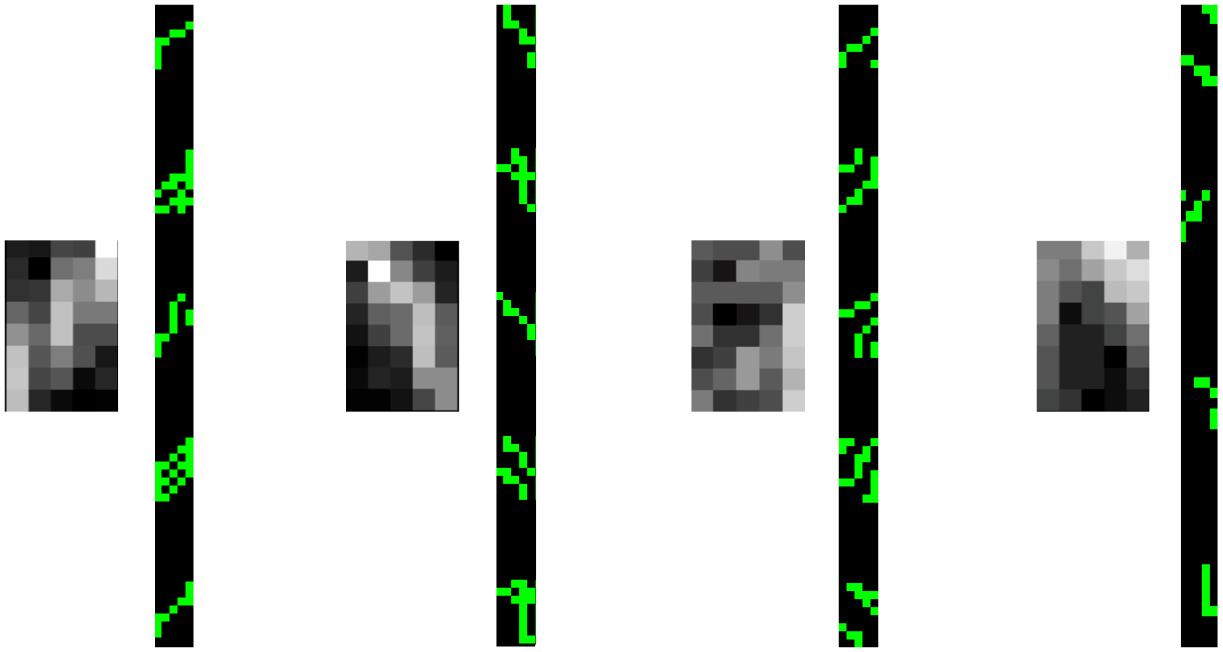
\includegraphics[width=0.8\textwidth]{hmm_example.png}
\end{center}
\caption{An example of training four HMMs to describe 200 observations of data.}
\label{fig:hmm_example}
\end{figure}

Figure~\ref{fig:hmm_example} shows an example of applying K-means clustering to Hidden Markov models.  The four models were trained from a five sensor neighborhood taken from the Brown Building Dataset.  The black bars show example observations while the large rectangles show a representation of the HMM trained for that data.  This run was performed on 200 observations and the above algorithm found these four HMMs to describe the data.  

Performing this type of clustering to train HMMs has shown considerable promise.  While we have not yet trained HMMs on residual data, we believe this approach will translate well and accurately capture activities due to the similarity of residual data to the raw data on which we have previously worked.\newline

\textbf{Time Series Mixture of Gaussians}

A mixture of Gaussians is a strongly supported stochastic data clustering technique used in activity recognition.  Traditionally, a mixture of Gaussians is implemented for either a one dimensional time series (CITE PAPER TO SUPPORT THIS) or for data vectors with no time element.  Here we combine the two approaches, creating a mixture of Gaussians for multi-dimensional time series data.  While this approach has not yet been implemented, based on the success of mixture of Gaussians in other domains, we expect good results.

The goal of mixture of Gaussians is to find a set of models which will maximize the log likelihood of the parameters of some models to the dataset.  Given dataset $\{x^{(i)}\}$ we maximize
\begin{equation}
\ell(\theta) = \sum_{i = 1}^{\bf M}log\{p(x^{(i)}|\theta)\}
\end{equation}
\noindent 
where ${\bf M}$ is the total number of time series instances.

The expectation maximization (EM) algorithm is commonly used to maximize dataset likelihood.  To use this algorithm we need to define a set of variables
\begin{equation}
w_{k}^{(i)} = p(z = k|x^{(i)})
\end{equation}
\noindent
where ${\bf K}$ is the total number of Gaussians to train and $k$ is an index of ${\bf K}$.  

The general equation for the likelihood of the models is: 
\begin{equation}
\label{eq:em_likelihood}
\ell(\theta|x) = \sum_{i = 1}^{{\bf M}}\sum_{k = 1}^{{\bf K}}w_{k}^{(i)}\log \{ \frac{p(x^{(i)}|z=k)p(z = k)}{w_{k}^{(i)}} \}
\end{equation}

In the traditional mixture of Gaussians algorithm each model is ostensibly a Gaussian.  To make this algorithm work with multi-dimensional time series, we define the models instead by
\begin{equation}
\label{eq:model}
p(x^{(i)}|z = k) = \prod_{n = 1}^{{\bf N}}\mathcal{N}_{n}(x^{(i)})
\end{equation}
\noindent
where ${\bf N}$ is the length of each time series instance.  Thus our model for each time series is ${\bf N}$ independent multivariate Gaussians.

Combining equations~\ref{eq:em_likelihood} and~\ref{eq:model} gives the following log likelihood
\begin{equation}
\label{eq:em_combined}
\ell(\theta|x) = \sum_{i = 1}^{{\bf M}}\sum_{k = 1}^{{\bf K}}w_{k}^{(i)}\{ \log\frac{p(z = k)}{w_{k}} + \sum_{n = 1}^{{\bf N}} \log \mathcal{N}_{n}(x^{(i)})\}
\end{equation}

\textbf{E-Step}
The E-step hardly changes from the traditional EM mixture of Gaussians algorithm.  We simply need to calculate 
\begin{equation}
w^{(i)}_{k} = p(z = k|x^{(i)})
\end{equation}

\textbf{M-Step}
For the maximization step, it is assumed that we know the values of $w_{k}^{(i)}$.  Thus, we need to maximize equation~\ref{eq:em_combined} with respect to $\mu$,  $\Sigma$, and $\theta$.
The results of these maximizations are given below:
\begin{equation}
\theta_{k} = \frac{1}{{\bf M}}\sum_{i = 1}^{{\bf M}}w_{k}^{(i)}
\end{equation}
\begin{equation}
\mu_{k, n} = \frac{\sum_{i = 1}^{{\bf M}}w_{k}^{(i)}x^{(i)}_{n}}{\sum_{i = 1}^{{\bf M}}w_{k}^{(i)}}
\end{equation}
\begin{equation}
\Sigma_{k, n} = \frac{\sum_{i = 1}^{{\bf M}}w_{k}^{(i)}(x^{(i)} - \mu_{k, n})(x^{(i)} - \mu_{k, n})^{\mathrm{T}}}{\sum_{i = 1}^{{\bf M}}w_{k}^{(i)}}
\end{equation}


%\subsubsection{Suffix Tree} 
%Suffix Trees offer another potential approach to activity modeling.  These trees are built from the suffixes of a given observation time series.  The final result is a tree where the potential subsequences within a time series are represented stochastically.  

%The primary advantage of a suffix tree over a HMM is in its ability to take into account a longer history of observations.  For example consider the observation sequence:

%\begin{equation}
%\{a, b, c, b, d, a, b, c\}
%\end{equation}

%In this sequence, observation $b$ is followed by either $c$ or $d$.  However the sequence $a, b$ is always followed by $c$.  This behavior may cause problems for a first order HMM, but suffix trees are able to handle longer sequences.  Training of suffix trees for activity recognition has been performed by \cite{Hamid2007} with some success however in noisy situations HMMs will typically out perform suffix trees.  

%We propose implementing suffix trees as a supplement to HMM or other activity models to be used in our final ensemble predictor.

%\subsection{Combination of Activities}
%As mention previously, we assume that at least some of the data is generated from a set of discrete activities.  This assumption is the motivation for our usage of activity models to aid in prediction.  We also assume that activities are additive.  A time series of residual observations may be made of up any combination of activities.  

%To show the need for combined activities consider the following example.  Given activities $a = \{6, 5, 4, 3, 2, 1\}$ and $b=\{3, 5, 2\}$ and the observation sequence $o = \{6, 5, 4, 6, 7, 3\}$ it is clear that no activity perfectly fits the observation sequence $o$.  However adding the activities  together with the proper time offset we get $o = o_{a,b} = \{a_1, a_2, a_3, a_4 + b_1, a_5 + b_2, a_6, b_3\}$.  It is possible to find a linear combination of the activities to reconstruct $o$.  

%This problem is roughly analogous to the subset-sum problem.  The differences are that we allow for a non-perfect matching and the constraints imposed by lining up time series instead of integers.  The subset sum problem is NP complete when allowing for every possible combination of activities.  In practice, we believe it is unlikely for their to be more than a few simultaneous activities occurring thus we can bound the potential number of combinations by searching for all combinations of k activities where k is likely to be 4 or less.  

%If an environment is complicated enough that the number of simultaneous activities is such that a brute force calculation of the potential combinations of activities becomes intractable, we will then look for more computationally feasible solutions based on methods used to solve the subset-sum problem.  However, until that problem presents itself, we propose searching for combinations of activities to best describe any observation sequence through brute force alone.

\subsection{Performance Metrics}
The final measure for forecasting performance is MAPE or MASE.  This measure encompasses the all steps of our algorithm.  It would be helpful to have a measure of performance for activities alone.  Because most activity recognition work has a classified dataset, the techniques commonly used, such as precision and recall, will not apply for our problem.  Ostensibly, a set of activity models which are both accurate and are identified with small amounts of data leads to greater forecasting accuracy as the earlier an activity model can be identified, the earlier its forecasts may be applied to final forecasting.  Thus, as a way to compare activity recognition techniques, it is important to know both the accuracy of the activity models and the time it takes to correctly identify the correct model for a given time series.

To calculate activity model accuracy the traditional mean squared error or root mean square cost functions should work well.  For calculating the time to identify the correct model we propose a measure defined here.  To calculate this we first define activity identification as:
\begin{equation}
\label{eq:activity_identification}
C(x) = \arg\max_{k} A_{k}(x) \ \forall k
\end{equation}
\noindent
where $x$ is a time series of length $M$ and $A_{k}(x)$ is the probability that time series $x$ corresponds to activity $k$.

Next, we introduce another term which we call an identification set.  This set is defined as:
\begin{equation}
\label{eq:identification_set}
c_M = \{C(x_{1:2}), C(x_{1:3}), ..., C(x_{1:M})\}
\end{equation}
\noindent
where $x_{i:j}$ represents all data from time offset $i$ to time offset $j$.  Notice that the length of $c$ will be equal to the length of the time series $M$.

Using the identification set, it is now possible to calculate the identification time.  
\begin{equation}
\label{eq:identification_time}
J(x) = \max_{i}\ \{i|c_{M}=c_{M-1}=,...,c_{M-i}\}
\end{equation}
\noindent
This measure calculates for a given time series the earliest time at which no misidentification occur.  The measure we are interested in is the average identification time for a set of activity models.

Using both activity model accuracy and identification time allows for a comparison of activity recognition techniques and determination of the number of activity models.  If too many activity models are trained then it is expected that training set activity accuracy will increase, but identification time will increase.  If too few activity models are trained, training set activity accuracy will decrease, but identification time will decrease.  Finding a balance between accuracy and classification time will be performed empirically. 

%Forecasting
\section{Forecasting Model}
To improve on the forecasts of the seasonal ARIMA model we attempt to forecast the error in the ARIMA model.   To forecast this error we want to use the forecasts of all trained activity models.  The approach that we propose to implement this forecasting is to use a Bayesian Combined Predictor (BCP) \cite{Petridis2001}.  A BCP is a method for combining the forecasts of multiple models given the probability for each model based on current observations and the probability of each model given a short history of observations.  The BCP is defined as:

\begin{equation}
\label{eq:model_prob}
p_{k}^{(t)} = p(k|x_{1:t}) = \frac{p_{k}^{t - 1} \cdot err(x_{t} - h_{k}(x^{1:t-1})}{\sum_{j=1}^{K}p_{j}^{t - 1} \cdot err(x^{(t)} - h_{j}(x_{1:t-1})}
\end{equation}
\noindent
where $p(Z=k|x)$ is the probability of model k given data x, $K$ is the total number of models, $h_{k}$ is the forecast from model $k$, and $err()$ is the probability mass function of the forecasting error for model $k$.  

Forecasting is then performed by finding the model which is most model likely describing the current activity and taking the forecast from that model.

\begin{equation}
\label{eq:prediction}
h_{k} = h_{k\ast} \ \ \ where \ \ k\ast = \arg\max_{1 \le k \le K} p_{k}^{(t)}
\end{equation}

If the forecasting error of each model is assumed to be Gaussian, calculating the BCP is relatively easy.  Also, because BCP will always select from a model to forecast, we introduce a null model $\sim N(0, \sigma^{2})$ which we represent as a Gaussian with zero mean and standard deviation $\sigma$ which is calculated from the seasonal ARIMA model.   

BCP resolves some of the problems present with multiple model forecasting.  Because research has shown \cite{Huynh2005} empirically that there exists no one model, feature space, or time scale that best describes all the possible activities, it is likely optimal to train models which incorporate different features and time scales.  BCP allows for forecasting with a heterogeneous mixture of models by allowing each model its own probability mass error function and history of readings.


